%
% Charset: utf8
% File type: Plain LATEX
% Content: This chapter describes the deployment of the Mini2440.
%
% Copyright Jürgen Beisert <jbe@pengutronix.de>, 2011
%
% This work is licensed under the Creative Commons Attribution 3.0 Unported License.
% To view a copy of this license, visit:
%           http://creativecommons.org/licenses/by/3.0/
% or send a letter to:
% Creative Commons, 444 Castro Street, Suite 900, Mountain View, California, 94041, USA.
%
% Refer the file CREDITS for all people working on this document.
%
% This file content will be part of the "OSELAS.BSP-Pengutronix-Mini2440-Quickstart.pdf"
%
% Note: This document uses some externaly defined LATEX commands. If you try to
% run LATEX only on this file it will fail due to the absense of these commands
% All these commands are starting with 'ptxdist'.
%

\section{Bring in the Bootloader Barebox}	\label{sec:deploying}

In order to make use of all possible boot sources the bootloader Barebox must
be installed into the Mini2440. This bootloader enables the following boot
sources:

\begin{itemize}
	\item NAND flash memory: This enables the Mini2440 to boot standalone
	and very fast
	\item SD/MMC card: This enables the user to change all relevant
	software parts very easy by changing the SD/MMC card
	\item Network: This is intended for easy development
\end{itemize}

What we need for this step:

\begin{itemize}
 \item a working network infrastructure
 \item host with network and USB capabilities
 \item a working TFTP server on our host
 \item some cables
 \begin{itemize}
  \item network
  \item USB-A to USB-B
  \item RS232
 \end{itemize}
 \item serial terminal running on our host
\end{itemize}

We assume here:

\begin{itemize}
 \item the directory of the TFTP server is \texttt{/tftpboot}
 \item network is already configured for the host and the target
       (refer section \ref{sec:networkadaptions})
 \item all connections are done (network, USB, serial)
 \item the serial terminal is able to handle 8 bits at 115200 Bd
\end{itemize}

To load the kernel and rootfs images, we first must load the new bootloader.
This is the trickiest part, as we need special tools on our host and the target.
Also, we may have to deal with confusing error messages.

First of all, we must change the \textbf{S2} switch on our Mini2440
to the \texttt{NOR} position to start the internal \textit{vivi} bootloader.
After switching on the Mini2440, the vivi bootloader will greet us
with:

\begin{ptxshell}[escapechar=|]{^}
##### FriendlyARM BIOS for 2440 #####
[x] bon part 0 320k 2368k
[v] Download vivi
[k] Download linux kernel
[y] Download root_yaffs image
[a] Absolute User Application
[n] Download Nboot
[l] Download WinCE boot-logo
[w] Download WinCE NK.bin
[d] Download & Run
[z] Download zImage into RAM
[g] Boot linux from RAM
[f] Format the nand flash
[b] Boot the system
[s] Set the boot parameters
[u] Backup NAND Flash to HOST through USB(upload)
[r] Restore NAND Flash from HOST through USB
[q] Goto shell of vivi
[i] Version: 1026-12
Enter your selection:
\end{ptxshell}

We want to use the \textit{vivi} bootloader to load the new Barebox bootloader
into the Mini2440's RAM. In order to do so, we need the size in bytes of
Barebox's binary:

\begin{ptxshell}[escapechar=|]{^}
|\$| ls -l |\ptxdistPlatformDir |images/barebox-image
-rw-r--r-- 1 jb user 147844 Jun 04 23:07 |\ptxdistPlatformDir |images/barebox-image
\end{ptxshell}

The size of this binary may differ in your case. In our case here it is
\textit{147844}.

With this size we instruct the \textit{vivi} bootloader to expect this number of
bytes from the USB and store it to the internal RAM. To do so, we enter
'\textit{q}' to enter vivi's shell. Then we start the download command.

\begin{ptxshell}[escapechar=|]{^}
Enter your selection: q
Supervivi> load ram 0x31000000 147844 u
\end{ptxshell}

Please consider the \textit{147844} number here. This number must be the same
as size of your Barebox image.

At this point of time many error messages can happen. The Mini2440
may output \texttt{USB host is not connected yet}. In this case disconnect
the USB cable again, powercycle the Mini2440 and try again.

At the host side, the system may not be able to enumerate the Mini2440
correctly. In this case also disconnect the Mini2440, powercycle it
and connect it again.

You can check that the host was able to enumerate the Mini2440 successfully by
issuing the \texttt{lsusb} command. If the following line occurs in the list,
the Mini2440 is successfully enumerated:

\begin{ptxshell}[escapechar=|]{^}
Bus 001 Device 023: ID 5345:1234 Owon PDS6062T Oscilloscope
\end{ptxshell}

Note: The bus and device number may differ in your case.

If the USB connection is up and working on both sides, we can start to push
the new bootloader into the target. This BSP comes with the required tool to do
so.

\begin{ptxshell}[escapechar=|]{^}
|\$| sudo |\ptxdistPlatformDir |sysroot-host/bin/usbpush |\ptxdistPlatformDir |images/barebox-image
\end{ptxshell}

If the transfer was successful, the \texttt{usbpush} host tool will output:

\begin{ptxshell}[escapechar=|]{^}
csum = 0x74f9
send_file: addr = 0x30000000, len = 0x00024124
\end{ptxshell}

At the target side we will see:

\begin{ptxshell}[escapechar=|]{^}
Now, Downloading [ADDRESS:31000000h,TOTAL:147854]
RECEIVED FILE SIZE:  147854 (144KB/S, 1S)
Downloaded file at 0x31000000, size = 147844 bytes
\end{ptxshell}

Note: The numbers shown above may be different then what you see.

After a successful transfer, we can now run the downloaded bootloader:

\begin{ptxshell}[escapechar=|]{^}
Supervivi>  go 0x31000000
go to 0x31000000
  argument 0 = 0x00000000
  argument 1 = 0x00000000
  argument 2 = 0x00000000
  argument 3 = 0x00000000
\end{ptxshell}

This will start the Barebox bootloader on the Mini2440, which will
greet us with:

\begin{ptxshell}[escapechar=|]{^}
barebox |\ptxBareboxRev |-mini2440-ptx-|\releasenumber| (July  13 2011 - 14:21:13)

Board: Mini 2440
NAND device: Manufacturer ID: 0xec, Chip ID: 0x76 (Samsung NAND 64MiB 3,3V 8-bit)
Bad block table found at page 131040, version 0x01
Bad block table found at page 131008, version 0x01
dm9000 i/o: 0x20000300, id: 0x90000a46
eth@eth0: got MAC address from EEPROM: FF:FF:FF:FF:FF:FF
refclk:    12000 kHz
mpll:     405000 kHz
upll:      48000 kHz
fclk:     405000 kHz
hclk:     101250 kHz
pclk:      50625 kHz
SDRAM1:   CL4@101MHz
SDRAM2:   CL4@101MHz
Malloc space: 0x33a00000 -> 0x33e00000 (size  4 MB)
Stack space : 0x339f8000 -> 0x33a00000 (size 32 kB)
envfs: wrong magic on /dev/env0
no valid environment found on /dev/env0. Using default environment
running /env/bin/init...

Hit any key to stop autoboot:  3
\end{ptxshell}

Stop the autoboot timeout by hitting any key. We are now in the shell
environment of Barebox. To update the NAND content in the next step we need
a working network first. One check is to show the current setting of the
network interface. You should see your own settings here, done in section
\ref{sec:networkadaptions}. Here is an example for a static network configuration:

\begin{ptxshell}[escapechar=|]{^}
mini2440:/ devinfo eth0
base  : 0x00000000
size  : 0x00000000
driver: none

Parameters:
          ipaddr = 192.168.1.240
         ethaddr = 00:04:f3:00:06:35
         gateway = 192.168.1.2
         netmask = 255.255.255.0
        serverip = 192.168.1.7
\end{ptxshell}

If you do not see appropriate values here and you are using the DHCP option, run
the \texttt{dhcp} command first:

\begin{ptxshell}[escapechar=|]{^}
mini2440:/ dhcp
DHCP client bound to address 192.168.1.27
\end{ptxshell}

If you do not use DHCP for network configuration, you must edit the file
\texttt{/env/config} in the Barebox environment.

\begin{ptxshell}[escapechar=|]{^}
mini2440:/ edit /env/config
\end{ptxshell}

Note: Barebox supports auto completion of commands, paths and filenames. Use
the well known TAB key.

Edit the lines beginning with \texttt{eth0.*} and give them appropriate values.
We can leave the editor by hitting CTRL-D to save our changes, or CTRL-C to
discard any change. If we want these new settings to be persistent, we can save
them now to NAND:

\begin{ptxshell}[escapechar=|]{^}
mini2440:/ saveenv
\end{ptxshell}

For further explanation about the default (compiled-in) Barebox environment
and the “user defined” Barebox environment in NAND, see section \ref{sec:bbenv}.

To make the new static network configuration work, we must execute the
\texttt{config} file again:

\begin{ptxshell}[escapechar=|]{^}
mini2440:/ . /env/config
\end{ptxshell}

Running the \texttt{devinfo eth0} command again should now show the values for
the network interface that you put in earlier. To check if it is really working,
try pinging other hosts:

\begin{ptxshell}[escapechar=|]{^}
mini2440:/ ping 192.168.1.7
host 192.168.1.7 is alive
\end{ptxshell}

In order to store the bootloader Barebox into the NAND, we can now use
some of the builtin features in Barebox.

First we must copy - at the host side - the Barebox image from the board support
package to the directory used by the TFTP server:

\begin{ptxshell}[escapechar=|]{^}
|\$| cp |\ptxdistPlatformDir |images/barebox-image /tftpboot/barebox-mini2440
\end{ptxshell}

Due to some scripts from the compiled-in environment and already setting up the
network, storing Barebox into the NAND is now very easy:

\begin{ptxshell}[escapechar=|]{^}
mini2440:/ update -t barebox -d nand
\end{ptxshell}

That's all. To boot using the new bootloader, we must now change the switch
\textbf{S2} back to the NAND position. Power cycle the Mini2440 or press its
reset button and the new bootloader will start.

After installing Barebox on the Mini2440 the hardest part is done. Now it's
time to decide about how to boot the Mini2440.

\section{How to Boot the Mini2440}	\label{sec:bootingmini2440}

Various methods are exist to bring up the Mini2440. The main difference is if
the Mini2440 can boot in a standalone manner or if it depends on some services
from another host via network.

To start the Mini2440 in a standalone manner it provides some local memory types
to store the relevant software parts.

\begin{itemize}
\item \texttt{NOR type flash memory} can be used to bring up the Mini2440. In
	this BSP NOR is used for the initial bootload of Barebox and as a
	fall-back or rescue bootloader. This allows the user to easily restore
	a "bricked" Mini2440.
\item \texttt{NAND type flash memory} provides enough memory space to hold all
	run-time relevant software parts. This board support package supports
	this memory type as one way to start the Mini2440 standalone.
\item \texttt{SD/MMC card memory} is a nice and easy way to deploy the run-time
	relevant software parts at the development host and simply booting
	the Mini2440 with it.
\end{itemize}

Note: All the mentioned boot methods below require Barebox as their bootloader.
The easiest way to get Barebox into the Mini2440 is via its internal NAND. So,
at least Barebox and its persistent environment has to be stored into the NAND
flash memory. The other parts (kernel and root filesystem) can be loaded from
all other supported media.

\subsection{NOR Type Flash Memory}

As the NOR type flash memory is not supported in this board support package,
we skip its explanation here.

\subsection{NAND Type Flash Memory}				\label{sec:nandflashmem}

This is the most common method to boot the Mini2440. It does not depend on
any external media or network connection. And it is also a fast method to
boot it.

To use the NAND flash as the boot media, this board support package creates
two files when running the last \texttt{ptxdist images} step:

\begin{itemize}
\item \texttt{\ptxdistPlatformDir images/linuximage} is the Linux kernel
	and must be stored in the corresponding NAND partition
\item \texttt{\ptxdistPlatformDir images/root.jffs2} contains the root filesystem
	and must be stored 'as is' in the corresponding NAND partition
\end{itemize}

\centerline{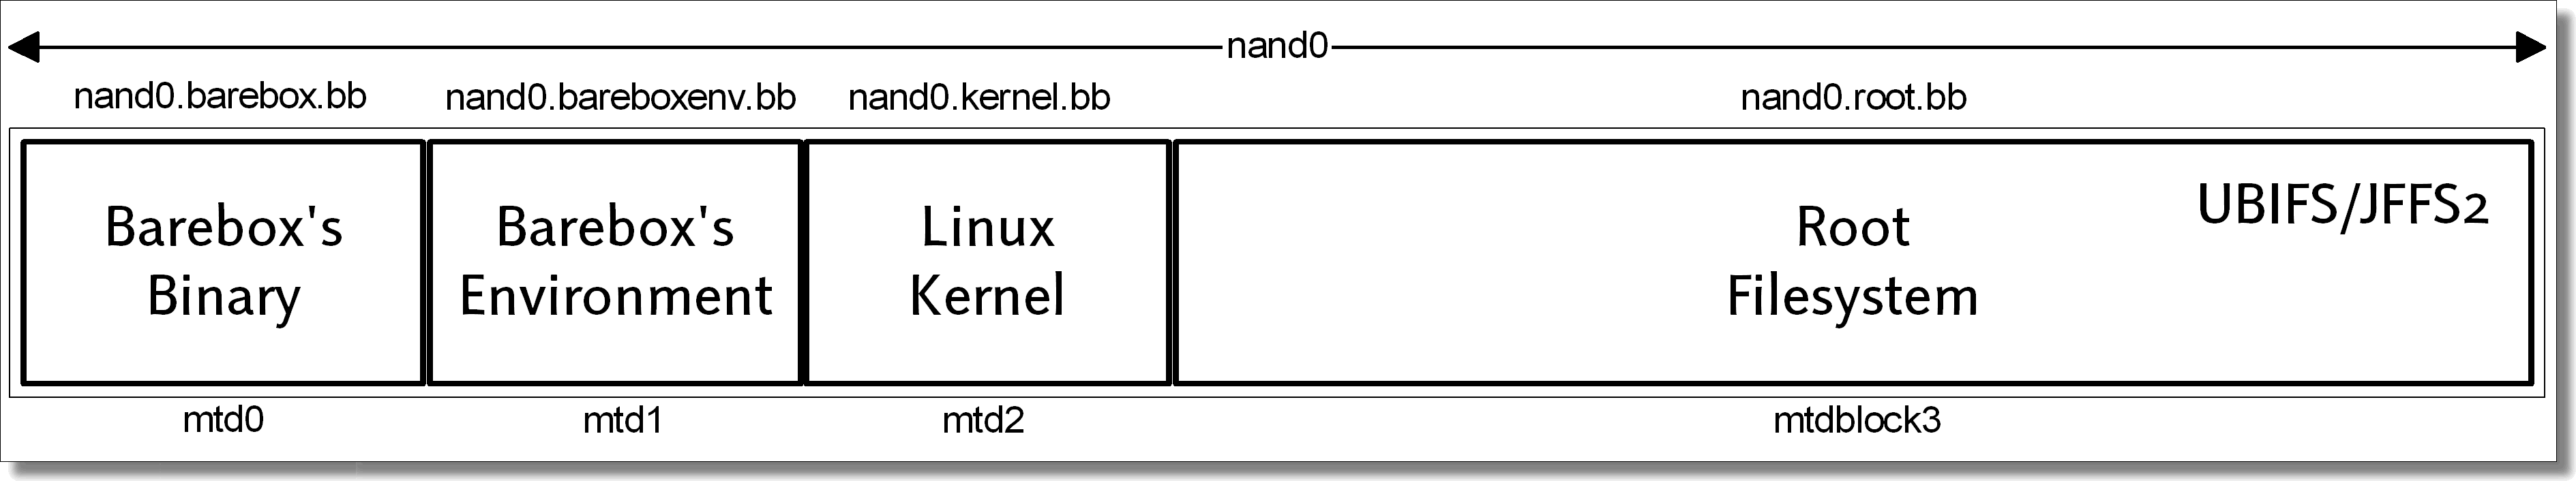
\includegraphics{OSELAS.BSP-Pengutronix-Mini2440/documentation/plain_sources/nand_partition.png}}

At our host's side:

\begin{ptxshell}[escapechar=|]{^}
|\$| cp |\ptxdistPlatformDir |images/root.jffs2 /tftpboot/root-mini2440.jffs2
|\$| cp |\ptxdistPlatformDir |images/linuximage /tftpboot/uImage-mini2440
\end{ptxshell}

Then we can run a script at the Mini2440's side to bring in the files into the
NAND memory:

\begin{ptxshell}[escapechar=|]{^}
mini2440:/ update -t rootfs -d nand
mini2440:/ update -t kernel -d nand
\end{ptxshell}

Corresponding setup in the Barebox's \texttt{/env/config}:

\begin{ptxshell}[escapechar=|]{^}
kernel_loc=nand
rootfs_loc=nand
\end{ptxshell}

Specific settings in \texttt{/env/config} for the NAND case:

\begin{ptxshell}[escapechar=|]{^}
rootfs_type=jffs2
rootfs_mtdblock_nand=3
kernelimage_type=uimage
\end{ptxshell}

With these settings Barebox will automatically load the kernel from the NAND
memory and instruct the kernel to also use the NAND memory for its root
filesystem. \texttt{rootfs\_mtdblock\_nand} defines the partition number in the
NAND memory the kernel should mount as its root filesystem. \texttt{rootfs\_type}
defines the used filesystem. \texttt{kernelimage\_type} defines the type of the
kernel image, to make Barebox aware how to extract it.

Start manually:

\begin{ptxshell}[escapechar=|]{^}
mini2440:/ boot nand
\end{ptxshell}

The manual start from the NAND memory requires the following specific settings
in the \texttt{/env/config}:

\begin{ptxshell}[escapechar=|]{^}
rootfs_mtdblock_type=jffs2
rootfs_mtdblock_nand=3
kernelimage_type=uimage
\end{ptxshell}

\subsection{SD/MMC Card Memory}

To have all run-time relevant parts on an SD/MMC card, some help from the
NAND type flash memory is required: the Barebox bootloader must be present
to be able to load the Linux kernel from the SD/MMC media.

To deploy the card we just partition it and create a filesystem on the second
partition.

To deploy the card we just partitionate it and create a filesystem on the second
partition. As this kind of media behaves like a regular hard disk, we can use
any filesystem we like. But there is still a risk: this kind of media uses flash
memory internally. And writing it often will destroy it over the time. That's why
at least a journaling filesystem might not be a good idea, as they tend to write
more data and more often as non journaling filesystems.

The generic Barebox's environment is prepared for the kernel in the first partition,
the root filesystem in the second partition and \textit{ext2} as the selected
filesystem. There is no policy to use it in this way, but any variation would
require some changes in the Barebox's default environment.

To use an SD/MMC card as the boot media, this board support package comes with
two files after the last \texttt{ptxdist images} step:

\begin{itemize}
\item \texttt{\ptxdistPlatformDir images/linuximage} is the Linux kernel
	and must be copied plainly into the first partition of the SD/MMC card
\item \texttt{\ptxdistPlatformDir images/root.tgz} contains the root filesystem
	and must be untared to the formatted second partition of the SD/MMC card
\end{itemize}

\centerline{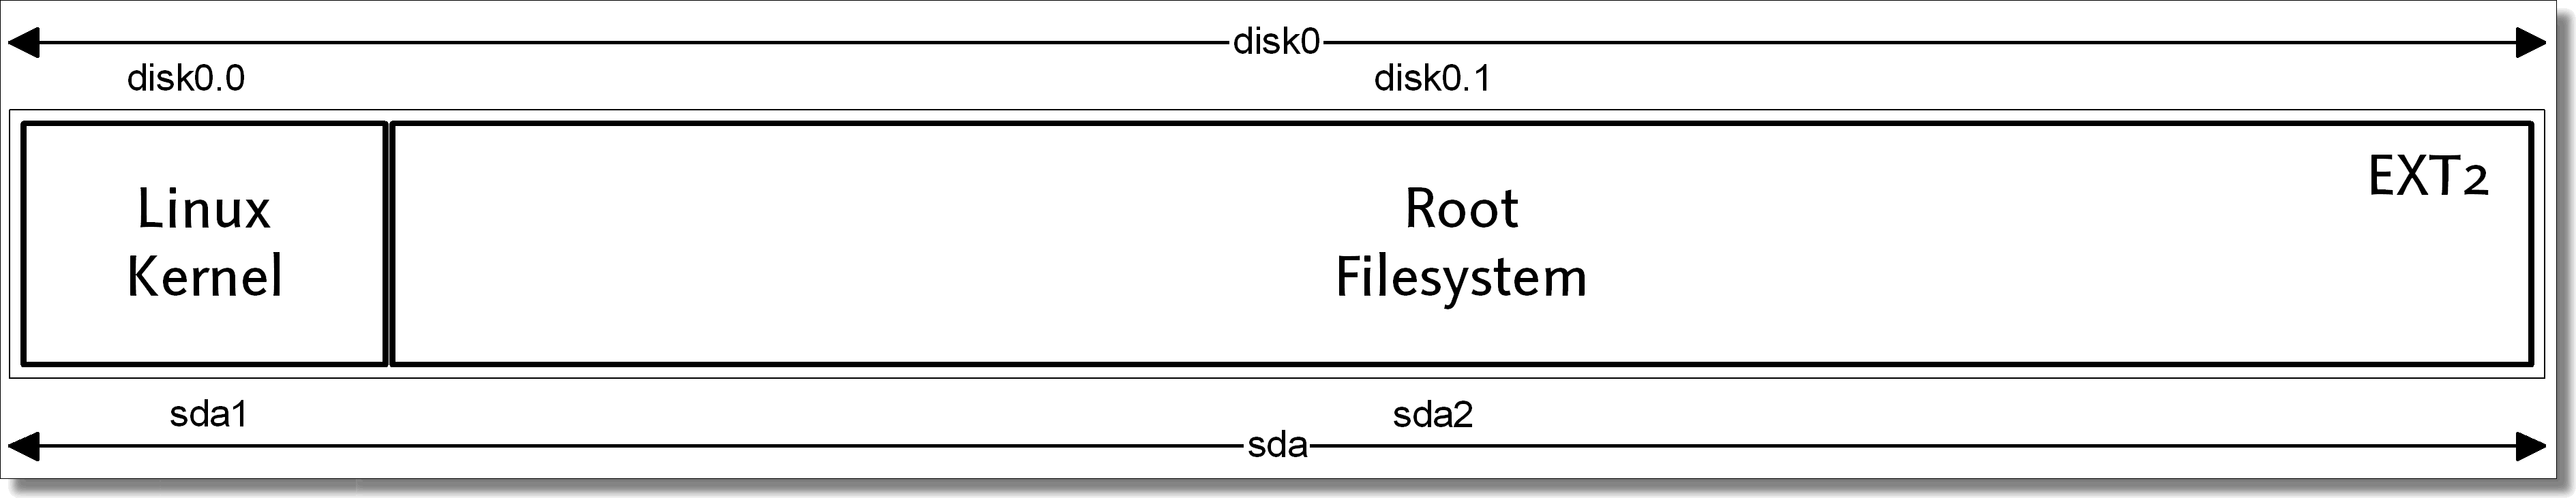
\includegraphics{OSELAS.BSP-Pengutronix-Mini2440/documentation/plain_sources/sd_card_partition.png}}

Note: The partition which contains the kernel image does not use any kind of
filesystem. So, the kernel's image is copied to the \textit{device}, not to
its \textit{filesystem}.

Persistent setup in the Barebox's \texttt{/env/config}.

\begin{ptxshell}[escapechar=|]{^}
kernel_loc=mmc
rootfs_loc=mmc
\end{ptxshell}

Specific settings in \texttt{/env/config} for the SD/MMC case:

\begin{ptxshell}[escapechar=|]{^}
rootfs_type=ext2
rootfs_mmc_part=2
kernel_mmc_part=0
kernelimage_type=uimage
\end{ptxshell}

With these settings Barebox will automatically load the kernel from the SD card
and instruct the kernel to also use the SD card as its root filesystem.
\texttt{kernel\_mmc\_part} defines the SD/MMC card's partition number to load the
kernel from. \texttt{rootfs\_mmc\_part} defines the partition on the SD/MMC card
the kernel should use as its root filesystem and \texttt{rootfs\_type}
defines the used filesystem. \texttt{kernelimage\_type} defines the type of the
kernel image, to make Barebox aware how to extract it.

Start manually:

\begin{ptxshell}[escapechar=|]{^}
mini2440:/ boot mmc
\end{ptxshell}

The manual start from the SD/MMC card requires the following specific settings
in the \texttt{/env/config}:

\begin{ptxshell}[escapechar=|]{^}
rootfs_type=ext2
rootfs_mmc_part=2
kernel_mmc_part=0
kernelimage_type=uimage
\end{ptxshell}

\subsection{Network Memory}				\label{sec:networkmem}

Using the network based method to boot the Mini2440 is more dedicated for
development. It simplifies replacing software in the kernel and root filesystem.
Also, the development cycle time can be reduced, with fewer opportunities for
making errors. All run-time relevant software parts are still
part of the development host in this case and can be easily changed on the
host and are instantly visible at the target's side.

To use the network based method this board support package creates the
following parts:

\begin{itemize}
\item \texttt{\ptxdistPlatformDir images/linuximage} is the Linux kernel
	and must be copied to the NFS or TFTP exported directory with a
	name the target expect it (in our case here for example
	\texttt{uImage-mini2440})
\item \texttt{\ptxdistPlatformDir root/} contains the root filesystem
	to be exported via NFS
\end{itemize}

\centerline{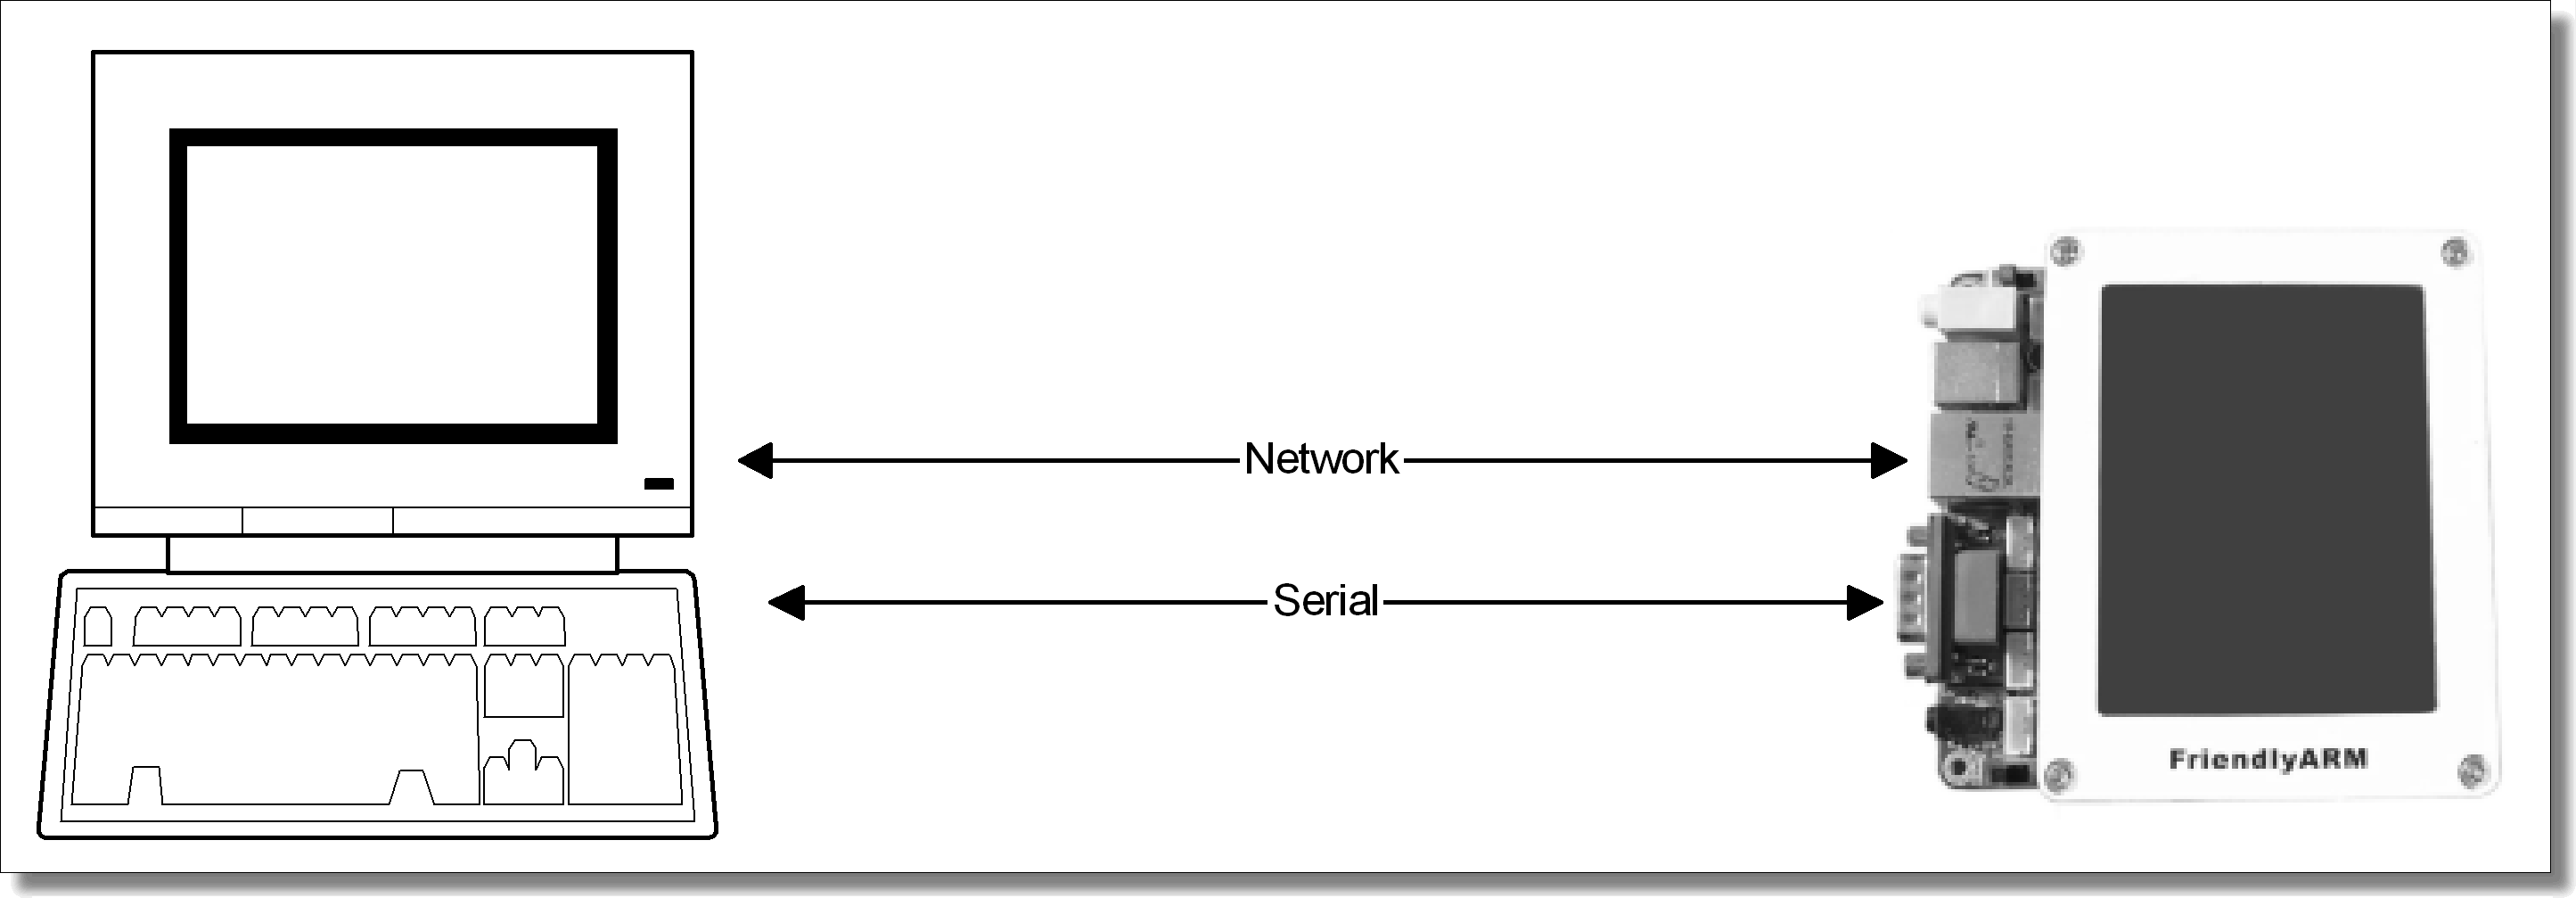
\includegraphics{OSELAS.BSP-Pengutronix-Mini2440/documentation/plain_sources/nfs_root.png}}

Persistent setup in the Barebox's \texttt{/env/config}.

Using the TFTP protocol for downloading the kernel:

\begin{ptxshell}[escapechar=|]{^}
kernel_loc=tftp
rootfs_loc=net
\end{ptxshell}

Specific settings in \texttt{/env/config} for the TFTP case:

\begin{ptxshell}[escapechar=|]{^}
kernelimage=uImage-mini2440
kernelimage_type=uimage
nfsroot="/path/to/nfs/root"
\end{ptxshell}

With these settings Barebox will automatically load the kernel with the name
\texttt{kernelimage} via network from a TFTP server and instruct it to use
the path given in \texttt{nfsroot} as its root filesystem.
\texttt{kernelimage\_type} defines the type of the kernel image, to make
Barebox aware how to extract it.

Using the NFS protocol for downloading the kernel:

\begin{ptxshell}[escapechar=|]{^}
kernel_loc=nfs
rootfs_loc=net
\end{ptxshell}

Specific settings in \texttt{/env/config} for the NFS case:

\begin{ptxshell}[escapechar=|]{^}
kernelimage=uImage-mini2440
kernelimage_type=uimage
nfsroot="/path/to/nfs/root"
\end{ptxshell}

With these settings Barebox will automatically load the kernel with the name
\texttt{kernelimage} via network from a NFS server and instruct it to use
the path given in \texttt{nfsroot} as its root filesystem.
\texttt{kernelimage\_type} defines the type of the kernel image, to make
Barebox aware how to extract it.

Start manually and download the kernel via TFTP:

\begin{ptxshell}[escapechar=|]{^}
mini2440:/ boot tftp
\end{ptxshell}

The manual start from a TFTP server requires the following specific settings
in the \texttt{/env/config}:

\begin{ptxshell}[escapechar=|]{^}
kernelimage=uImage-mini2440
kernelimage_type=uimage
nfsroot="/path/to/nfs/root"
\end{ptxshell}

Start manually and download the kernel via NFS:

\begin{ptxshell}[escapechar=|]{^}
mini2440:/ boot nfs
\end{ptxshell}

The manual start from an NFS server requires the following specific settings
in the \texttt{/env/config}:

\begin{ptxshell}[escapechar=|]{^}
kernelimage=uImage-mini2440
kernelimage_type=uimage
nfsroot="/path/to/nfs/root"
\end{ptxshell}

\subsection{Adaptions}

As mentioned above all settings are based on changes in a simple text file.
Whenever we run the 'boot' command, the script in \texttt{/env/bin/boot} is
called. So, adaptions can be made in \texttt{/env/config} to use one of the
supported boot methods in \texttt{/env/bin/boot}. For more complicated
scenarious also the \texttt{/env/bin/boot} can be changed. As it's a simple
shell script, it's very easy to adapt it to different requirements.

% --------------------------

\section{Updating the Mini2440}	\label{sec:updating}

Note: This section is for the boot method \textit{NAND Type Flash Memory}
(refer section \ref{sec:nandflashmem}).

At any time it's possible to update any of the software components
running on the Mini2440.

\begin{itemize}
	\item the bootloader Barebox
	\item Barebox's persistent environment
	\item the Linux kernel
	\item the kernel's root filesystem
\end{itemize}

\subsubsection{Updating the Bootloader}

Most of the time there is no further need to re-flash the bootloader and its
persistent environment. After it was setup once, it does its work "in the
background". But nevertheless there could be the need to update the bootloader
due to feature additions or bug fixes. If the current Barebox bootloader is
still working, its replacement can be done by using the existing bootloader.
This assumes that the network is still functioning. In this case, a simple

\begin{ptxshell}[escapechar=|]{^}
|\$| cp |\ptxdistPlatformDir |images/barebox-image /tftpboot/barebox-mini2440
\end{ptxshell}

provides the updated bootloader binary via TFTP and a

\begin{ptxshell}[escapechar=|]{^}
mini2440:/ update -t barebox -d nand
\end{ptxshell}

will do the job at the target side. After starting this command, do not disturb!
This is a critical update process. Because, for a short period of time the
NAND flash is erased, with no bootloader present. But don't panic: Unless a
power fail or a target reset happens, this command can be repeated if the
first run failed.

\subsubsection{Updating the Persistent Environment}

% I'm unsure how useful it is: Assuming the current environment is broken, I
% guess also the network setup is broken. So, loading via TFTP maybe is
% impossible.
% Idea:
% Maybe we should think about disasters a user can happen, and how to bring
% back life into her/his Mini2440 in this case

Updating the persistent environment is also possible. A simple

\begin{ptxshell}[escapechar=|]{^}
|\$| cp |\ptxdistPlatformDir |images/barebox-default-environment /tftpboot/barebox-default-environment-mini2440
\end{ptxshell}

provides the updated environment via TFTP and a

\begin{ptxshell}[escapechar=|]{^}
mini2440:/ update -t bareboxenv -d nand
\end{ptxshell}

will do the job. Note: This new persistent environment will be used at the next
system start.

If the persistent environment is broken, there is a second method to restore a
working environment: that is, using the compiled in default environment which
comes with Barebox.
To force the usage of the compiled in default environment, just erase the
current one in the NAND flash memory and reset the target (or run the
\texttt{reset} command).

\begin{ptxshell}[escapechar=|]{^}
mini2440:/ erase /dev/bareboxenv.bb
mini2440:/ reset
\end{ptxshell}

Now, Barebox will stumble about the empty partition and then fall back to its
compiled-in environment version. This can now be changed by editing the files
in \texttt{env/} and then saved back to the NAND flash memory with the command

\begin{ptxshell}[escapechar=|]{^}
mini2440:/ saveenv
\end{ptxshell}

\subsubsection{Updating the Linux Kernel}

Changing the Linux kernel configuration can be quite dynamic, especially while
the developer is trying different kernel configurations. Updating this part
happens in the same way like the other parts. Providing the Linux kernel via
TFTP:

\begin{ptxshell}[escapechar=|]{^}
|\$| cp |\ptxdistPlatformDir |images/linuximage /tftpboot/uImage-mini2440
\end{ptxshell}

and running the update script at the target's side:

\begin{ptxshell}[escapechar=|]{^}
mini2440:/ update -t kernel -d nand
\end{ptxshell}

\subsubsection{Updating the Root Filesystem}

And last, but not least, updating the root filesystem. Same procedure:

\begin{ptxshell}[escapechar=|]{^}
|\$| cp |\ptxdistPlatformDir |images/root.jffs2 /tftpboot/root-mini2440.jffs2
\end{ptxshell}

and running the update script at the target's side:

\begin{ptxshell}[escapechar=|]{^}
mini2440:/ update -t rootfs -d nand
\end{ptxshell}

% the following text should occur somewhere else, where it is more useful (?)
By the way: the \texttt{update} command is not a real command built into
Barebox. Its a simple shell script coming from the persistent environment.
If one has different update scenarios she/he can change or adapt this script.
Changing this behaviour can be done without touching Barebox's source code.

%
% Ideas:
% - Add info about how to test the Barebox written to the NAND (if it was
%   successful)
% - Add info on how to check the downloaded file is the correct one
% - maybe some comment about <erase /dev/nand0> and the use of <reset>
% - if you don't change anything using the edit command do you need to <saveenv>?  With
%   u-boot, most tutorials suggested a <saveenv>
% - What is dangerous about a <printenv>?
